\chapter{Magnetophoretic mobility}\label{ch:magnetophoretic_mobility}
%\chapter{Magnetophoresis}\label{ch:magnetophoresis}

%The increasing interest in single-cell analysis and the rapidly improving sensitivity of molecular biology methods in applications to single-cell genome, transcriptome and signalling analysis put a special emphasis on high quality, high volume, and relatively inexpensive cell separation methods such as those potentially provided by free-flow magnetophoresis (see Chapter~\ref{ch:fundamentalsOfMagnetophoresis}).

%Due to the increasing interest in magnetic particles have also gained an , different low cost and easily functionalizable microparticles are now commercially available from various manufacturers. Depending on their fabrication process, the different magnetic particles have slightly different magnetic composition, and thus differ in their magnetic behaviour. 


\section{Introduction}
\label{sec:introductionMagneticParticle}
In Chapter~\ref{ch:chapter2_theory}, the concept of magnetophoretic mobility was introduced as a fundamental property of a particle or cell and is equally applicable to materials that are diamagnetic, paramagnetic, or ferromagnetic, depending on the relationship between the applied field and the particle's susceptibility. Magnetophoretic mobility is the basic concept which enables the design of magnetic separation systems and provides a tool for the operation and evaluation of the magnetic separation process.

The increasing interest in using magnetic beads as carriers to perform cell separation tasks has also fuelled the industry of magnetic particles. Different low cost and easily functionalizable microbeads are now commercially available from various manufacturers. However, depending on their fabrication process, and the variability in these processes, the magnetic beads can vary significantly in respect of their material properties (e.g. size distribution or iron content). The extend to which beads deflect when being exposed to an external nonhomogeneous magnetic field highly depends on these properties (see Equation~\ref{eqn:terminalVelocity}). This makes the full control of single bead trajectories in free-flow magnetophoresis highly sensitive to small variations of intrinsic parameters. In order to have a separation device with high collection efficiency and discrimination it is essential to know the \textit{magnetic responsiveness} of the magnetic beads. 

As explained in Section~\ref{sec:theoryOfMagnetophoresis}, Equation~\ref{eqn:terminalVelocity} can be split into two independent terms, magnetophoretic mobility $\nu_{p}$ and magnetophoretic driving force $S$, given in Equation~\ref{eqn:magnetophoreticMobility} and Equation~\ref{eqn:magnetophoreticDrivingForce}. Previous work on free-flow magnetophoresis attempted to keep $S$ constant over the distance the particle travelled in order to have a constant magnetic migration velocity $\mathbf{u}_{p}$ and thus improved control of the particle movement~\cite{Zborowski1999,Zborowski2002,Derks2010}. A challenging task, however, is to find the exact value of the particle's magnetophoretic mobility $\nu_{p}$, since it depends on multiple material properties and is therefore highly dependent on the particle manufacturer. Different values for the magnetic susceptibility of iron oxide particles can be found in the literature~\cite{Clark1991,Hunt1995,Gupta2005}. Researchers have attempted to characterize the magnetic properties of the micron-sized beads directly; Fonnum \etal~\cite{Fonnum2005} as well as Shevkoplyas \etal~\cite{Shevkoplyas2007} determined the beads' magnetic response based on their magnetization curves (hysteresis loops). A different approach was used by Zborowski~\cite{Zborowski2002} and also H\"afeli~\cite{Haefeli2005}, where they measured the magnetophoretic velocity, using cell tracking velocimetry (CTV), to then work out the magnetophoretic mobility of single magnetic beads and their magnetic susceptibility. Yet, it is highly desirable to arrive at a definition of the magnetophoretic mobility as a property that is independent of a particular magnetic system and provides means of calculating motion of a magnetic particle for any field geometry.

Given the importance of the magnetophoretic mobility, the following chapter will describe a method to experimentally evaluate the magnetophoretic mobility of single superparamagnetic beads using a CTV system. Additionally, the magnetic susceptibility of the beads is measured using a superconducting quantum interference device (SQUID). In this study, five different types of magnetic beads from two different manufacturers (Table~\ref{tab:particleType}) are investigated and representative measures including mathematical relationships will be provided.

\begin{table}[htb]
\begin{center}
\caption[Physical characteristics of the five tested bead types]{Physical characteristics of magnetic beads: density, iron content and diameter ($d_{M}$) as stated by the manufacturer~\cite{chemicellConversation,dynabeads2015}. The diameter ($d_{p}$) is independently measured for comparison, by dynamic light scattering$^{(1)}$ or by analysing scanning electron microscopy$^{(2)}$ images.}
\vspace{1ex}
\label{tab:particleType}
\begin{tabular}{llcccc}
\hline
Bead & Manufacturer & Density & Iron content & \multicolumn{2}{c}{Diameter} \\
type && [$g/c$m$^{3}$] & [wt. $\%$] & $d_{M}$ [$\mu$m] & $d_{p}$ [$\mu$m]  \\
\hline
ScreenMAG	& Chemicell & $2.25$ & $40$ & $1.0$  & $0.77\pm0.42^{(1)}$ \\
SiMAG		& Chemicell & $2.25$ & $40$ & $1.0$  & $1.12\pm0.97^{(1)}$ \\
MyOne 		& Dynabeads & $1.8$  & $26$ & $1.05$ & $1.05\pm0.03^{(2)}$ \\
M280 		& Dynabeads & $1.4$  & $12$ & $2.8$  & $2.79\pm0.05^{(2)}$ \\
M270 		& Dynabeads & $1.6$  & $14$ & $2.8$  & $2.75\pm0.07^{(2)}$ \\ 
\hline
\end{tabular}
\end{center}
\end{table}

%The particles' multi-phase structure, described in Section~\ref{sec:superparamagneticMicroparticles}, as well as their superparamagnetic properties has been verified by Fonnum \etal~\cite{Fonnum2005} for the Dynabeads particles and confirmed by Chemicell GmBH for their particles~\cite{chemicellConversation}.

%A number of magnetometer devices can be used to measure the magnetic susceptibility of materials, such as Gouy and Faraday balances, and the superconducting quantum interference device (SQUID). While accurate, these devices only provide bulk measurements of materials and particles

\section{Magnetophoretic mobility of superparamagnetic beads}\label{sec:magnetophoreticMobilityOfSuperparamagneticParticles}
To compare the mobility of different single beads, their drift velocities in stationary fluid (deionized water) is observed, similar to the work of H\"{a}feli \etal~\cite{Haefeli2013}. Unlike Ref~\cite{Haefeli2013} where beads are kept at a constant distance from the magnet, in this work the magnetophoretic velocity is optically measured at different distances away from the magnet. This new approach allows evaluation of magnetic field dependence of the bead's properties.

The magnetophoretic movements of single magnetic beads in an observation chamber are observed under an optical microscope. The observation chamber used (see Section~\ref{subsec:microfluidicCountingSlide}), has a counting grid etched to its surface, which helped determine the viewing location of the beads within the observation chamber as well as the distance to the magnet. The distance $d_{m}$ between the bar magnet and the counting chamber can be adjusted and the magnetically induced velocity has been measured for the magnet positioned at $10$ mm, $12$ mm, $14$ mm and $16$ mm away from the counting grid. These four positions will also be referred to as A, B, C and D, respectively. Note, that $d_{m}$ describes the distance to the magnet's surface. A schematic diagram of this experimental setup is depicted in Figure~\ref{fig:magnetophoreticMobilityExperimentSchematic}. For a more detailed description of the experiment see Section~\ref{sec:magnetophoreticMobilityExperiment} in Chapter~\ref{ch:experiments}.

\begin{figure}[htb]
\centering
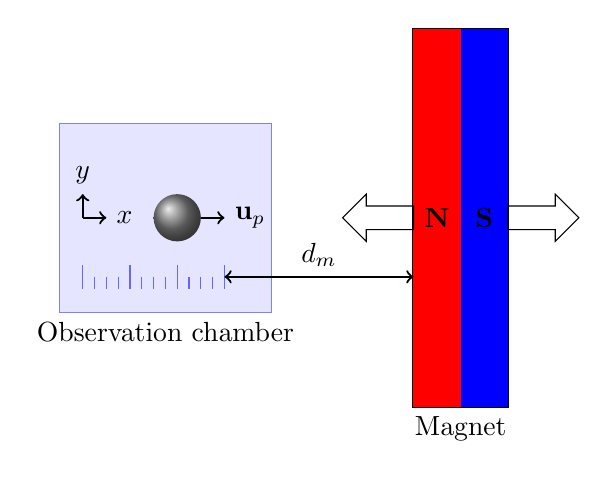
\begin{tikzpicture}[scale=0.6]
	\filldraw[color=blue!50!, fill=blue!10] (-2.5,-2) rectangle (2,2);
	\node[anchor=north] at (-0.25,-2) {Observation chamber};
	
	\draw[->,thick] (-2,0) -- (-1.5,0)node[anchor=west]{$x$};
	\draw[->,thick] (-2,0) -- (-2,0.5)node[anchor=south]{$y$};
	
	\draw[color=blue!60!](-2,-1.5) -- (-2,-1); 
	\draw[color=blue!60!](-1.75,-1.5) -- (-1.75,-1.25); 
	\draw[color=blue!60!](-1.5,-1.5) -- (-1.5,-1.25); 
	\draw[color=blue!60!](-1.25,-1.5) -- (-1.25,-1.25); 
	\draw[color=blue!60!](-1,-1.5) -- (-1,-1); 
	\draw[color=blue!60!](-0.75,-1.5) -- (-0.75,-1.25); 
	\draw[color=blue!60!](-0.5,-1.5) -- (-0.5,-1.25); 
	\draw[color=blue!60!](-0.25,-1.5) -- (-0.25,-1.25); 
	\draw[color=blue!60!](0,-1.5) -- (0,-1); 
	\draw[color=blue!60!](0.25,-1.5) -- (0.25,-1.25); 
	\draw[color=blue!60!](0.5,-1.5) -- (0.5,-1.25); 
	\draw[color=blue!60!](0.75,-1.5) -- (0.75,-1.25); 
	\draw[color=blue!60!](1,-1.5) -- (1,-1); 
	
  	\shade[ball color=gray] (0,0) circle (0.5);
  	\draw[->,thick] (0.5,0) -- (1.0,0) node[anchor=west] {$\mathbf{u}_{p}$};

  	\draw[thick](5,-4) rectangle (7,4);
  	
  	\fill[red] (5,-4) rectangle (6,4)node[black,font=\bf,pos=.5]{N};
  	\fill[blue] (6,-4) rectangle (7,4)node[black,font=\bf,pos=.5]{S};
	\node[anchor=north] at (6,-4) {Magnet};
	
	\draw(7,0.25) -- (8,0.25) -- (8,0.5) -- (8.5,0) -- (8,-0.5) -- (8,-0.25) -- (7,-0.25) -- cycle;
	\draw(5,0.25) -- (4,0.25) -- (4,0.5) -- (3.5,0) -- (4,-0.5) -- (4,-0.25) -- (5,-0.25) -- cycle;
	
  	\draw[<->,thick] (1,-1.25) -- node[anchor=south]{$d_{m}$} (5,-1.25);
\end{tikzpicture}
\caption[Schematic of experimentally used particle velocity tracking setup]{Schematic drawing showing the experimental setup used to determine the magnetically induced velocity of magnetic particles. The distance $d_{m}$ is varied step wise from $10$ mm to $16$ mm with a step size of $2$ mm. The figure shown here is not drawn to scale. The experimental setup can be seen in Section~\ref{sec:magnetophoreticMobilityExperiment}.}
\label{fig:magnetophoreticMobilityExperimentSchematic}
\end{figure}

The beads are tracked moving in the $x$ direction towards the magnet over a distance of $55$ $\mu$m, which is equivalent to one traverse of the field of view of the microscope camera. The magnetically induced velocity of single beads has been measured for each bead type in Table~\ref{tab:particleType} and for all four magnet positions. Beads travelling at the top or the bottom of the observation chamber are discarded in the measurement, to avoid including data from beads that are clearly interacting with the chamber surface. Also bead agglomerations have been ignored from this particular analysis. 

The magnet dimensions are much larger than the observation chamber. Thus, a uniform magnetic field along the width ($y$ direction) and height ($z$ direction) of the observation chamber is assumed and edge effects can safely be neglected. The magnetic field of the bar magnet is investigated in the next section.

\subsection{Properties of the static magnetic field}
The magnetic flux density of the bar magnet, under which the particles are influenced in the observation chamber, was simulated and measured to confirm its magnetic field (see Section~\ref{sec:magneticForceMeasurement}). The magnetic flux density map of the bar magnet is shown in Figure~\ref{fig:barMagnetFluxDensityMap}.

\begin{figure}[htb]
   \centering
   \includegraphics[width=0.7\textwidth]{img/chapters/chapter_4_magnetophoresis/magneticFieldBarMagnet.pdf}
   \caption[Magnetic flux density map of a N42 Neodymium bar magnet]{Modelling of the magnetic field generated by a N42 Neodymium magnet ($42\times8\times10$ mm) simulated in FEMM. The red box shows the position of the observation chamber and the two (open) arrows indicate that the magnet was attached to a movable stage.}
   \label{fig:barMagnetFluxDensityMap}
\end{figure}

Figure~\ref{fig:barMagnetFluxDensityOverDistance} shows how the magnetic flux density decays when moving away from the magnet surface along its centre line. The magnetic flux density is measured using a Hall probe and plotted on a log-linear graph to determine if the behaviour is exponential. The two straight line fits in Figure~\ref{fig:barMagnetMagneticFluxOverDistance_log_two} reveal that the data points are best modelled as two separate exponential functions, as determined by the gradient of the two straight lines. From this observation an empirical formula has been derived and compared to the ANSYS model. All three curves show a good agreement, as given in Figure~\ref{fig:barMagnetMagneticFluxOverDistance_log}, and confirms that the more computationally convenient empirical formula is a good approximation to the magnetic field.

\begin{figure}[htb]
	\centering
    \begin{subfigure}[b]{0.48\textwidth}
		\includegraphics[width=\textwidth]{img/chapters/chapter_4_magnetophoresis/barMagnetMagneticFluxOverDistance_two_exp1.eps}
         \caption{}  
		\label{fig:barMagnetMagneticFluxOverDistance_log_two}            
	\end{subfigure}
	\hfill
    \begin{subfigure}[b]{0.48\textwidth}
		\includegraphics[width=\textwidth]{img/chapters/chapter_4_magnetophoresis/barMagnetMagneticFluxOverDistance.eps}
         \caption{}    
		\label{fig:barMagnetMagneticFluxOverDistance_log}            
	\end{subfigure}
    \caption[Magnetic flux density of a N42 Neodymium bar magnet along its centre line]{Characterization of the magnetic flux density of a N42 Neodymium bar magnet ($42\times8\times10$ mm) in logarithmic and linear form. (a) The flux density measurement is fitted with two individual exponential curves and plotted on a logarithmic scale. (b) The flux density measurement is compared to the ANSYS simulation and a fitted function with two exponential terms and plotted on a linear scale. The measurement is taken along the centre line of the magnet, starting at the surface of the magnet to $48$ mm away, with a step size of $0.1$ mm. The error bars are calculated by taking the standard deviation of $14$ independent measurements at specific distances away from the magnet surface.}
        \label{fig:barMagnetFluxDensityOverDistance}
\end{figure}

In the region of interest, which is within a distance of $d_{m}=10$ mm to $d_{m}=16$ mm away from the magnet surface, the flux density is found to drop from $70$ mT to $38$ mT and the corresponding flux gradient was found to change from $8.3$ mT/mm to $3.4$ mT/mm, respectively. Within this region of interest, the fitted exponential curve is a good approximation to the measurements, as shown in Figure~\ref{fig:barMagnetFluxDensityOverROI}. The difference between the measurement and the fitted line in the area of interest was found to be no more than $0.6\%$. The different positions of interest are labelled with A, B, C and D. The labels correspond to $d_{m} = 10$ mm, $d_{m} = 12$ mm, $d_{m} = 14$ mm and $d_{m} = 16$ mm, respectively.

\begin{figure}[htb]
   \centering
   \includegraphics[width=0.7\textwidth]{img/chapters/chapter_4_magnetophoresis/barMagnetMagneticFluxOverROI_in_mT.eps}
   \caption[Magnetic flux density of a N42 Neodymium bar magnet around the region of interest]{Characterization of the magnetic flux density of a N42 Neodymium magnet ($42\times8\times10$ mm) between $10$ mm and $16$ mm away from the magnet surface. The letters A, B, C and D indicate the positions at which the magnetophoretic velocity of the particles are measured. The four positions are equivalent to $d_{m} = 10$ mm, $d_{m} = 12$ mm, $d_{m} = 14$ mm and $d_{m} = 16$ mm, respectively.}
   \label{fig:barMagnetFluxDensityOverROI}
\end{figure}

Ideally, the magnetophoretic driving force $S$ (see Equation~\ref{eqn:magnetophoreticDrivingForce}), which is the product of the magnetic $\mathbf{B}$ field and the field gradient $d\mathbf{B}/dx$, would be constant since this implies that the velocity of the magnetically attracted beads will be constant too. This is not possible with the setup used here, due to the shape and small size of the magnet. However, the magnetophoretic driving force can be approximated to be constant across the field of view ($55$ $\mu$m) since the maximum change in the magnetic field strength at the different magnet positions $d_{m}$ is only $1.5\%$, and can thus be neglected. 

%Figure~\ref{fig:changeOfMagnetophoreticDrivingForceAtDifferentDistances} shows the change of the magnetic driving force across the observed field of view (gray area).
%
%\begin{figure}[htb]
%        \centering
%        \begin{subfigure}[b]{0.48\textwidth}
%                \includegraphics[width=\textwidth]{img/chapters/chapter_4_magnetophoresis/barMagnetMagneticDrivingForceOverROI_pos1.png}
%                \caption{Position: A ($d_{m} = 10$ mm)}  
%        \end{subfigure}
%        \begin{subfigure}[b]{0.48\textwidth}
%                \includegraphics[width=\textwidth]{img/chapters/chapter_4_magnetophoresis/barMagnetMagneticDrivingForceOverROI_pos2.png}
%                \caption{Position: B ($d_{m} = 12$ mm)}                
%        \end{subfigure}
%        \begin{subfigure}[b]{0.48\textwidth}
%                \includegraphics[width=\textwidth]{img/chapters/chapter_4_magnetophoresis/barMagnetMagneticDrivingForceOverROI_pos3.png}
%                \caption{Position: C ($d_{m} = 14$ mm)}  
%        \end{subfigure}
%        \begin{subfigure}[b]{0.48\textwidth}
%                \includegraphics[width=\textwidth]{img/chapters/chapter_4_magnetophoresis/barMagnetMagneticDrivingForceOverROI_pos4.png}
%                \caption{Position: D ($d_{m} = 16$ mm)}                
%        \end{subfigure}
%        \caption[Change of the magnetophoretic driving force at different distances away from magnet surface]{Change of the magnetophoretic driving force at the different position A, B, C and D, indicated in Figure~\ref{fig:barMagnetFluxDensityOverROI}. The gray area indicates the field of view which is $55$ $\mu$m in width.}
%        \label{fig:changeOfMagnetophoreticDrivingForceAtDifferentDistances}
%\end{figure}

\subsection{Size characterization of superparamagnetic beads}
The magnetophoretic mobility highly depends on the particle size. Therefore, the superparamagnetic beads are all imaged using standard SEM techniques (see Section~\ref{subsec:semImaging} in Chapter~\ref{ch:experiments}). The SEM images allow for a clear inspection of the beads' shape and size distribution. Figure~\ref{fig:semParticleImages} shows SEM images of each of the bead types used in this thesis. Further SEM images of the different bead types can be found in Appendix~\ref{sec:magneticBeadImaging}.

\begin{figure}
\begin{subfigure}[b]{0.48\linewidth}
\includegraphics[width=\linewidth]{img/chapters/chapter_4_magnetophoresis/screenMag.jpg}
\caption{Chemicell ScreenMAG}\label{fig:semImage_ScreenMag}
\end{subfigure}
\hfill
\begin{subfigure}[b]{0.48\linewidth}
\includegraphics[width=\linewidth]{img/chapters/chapter_4_magnetophoresis/siMag.png}
\caption{Chemicell SiMAG}\label{fig:semImage_SiMag}
\end{subfigure}
\begin{subfigure}[b]{0.48\linewidth}
\includegraphics[width=\linewidth]{img/chapters/chapter_4_magnetophoresis/myOne.png}
\caption{Dynabeads MyOne}\label{fig:semImage_MyOne}
\end{subfigure}
\hfill
\begin{subfigure}[b]{0.48\linewidth}
\includegraphics[width=\linewidth]{img/chapters/chapter_4_magnetophoresis/M280.png}
\caption{Dynabeads M280}\label{fig:semImage_M280}
\end{subfigure}
\begin{subfigure}[b]{0.48\linewidth}
\includegraphics[width=\linewidth]{img/chapters/chapter_4_magnetophoresis/M270.jpg}
\caption{Dynabeads M270}\label{fig:semImage_M270}
\end{subfigure}
\caption[SEM images of different superparamagnetic particles]{SEM images of superparamagnetic particles of different types and from different manufacturers. (a) and (b) show $1$ $\mu$m sized ScreenMAG and SiMAG beads by Chemicell. (c), (d) and (e) show $1$ $\mu$m MyOne, $2.8$ $\mu$m M280 and $2.8$ $\mu$m M270 Dynabeads, respectively, from Thermo Fisher Scientific. Note the irregular shape of the Chemicell beads compared to those supplied by Dynabeads.}
\label{fig:semParticleImages}
\end{figure}

A clear visual difference between the two manufacturers can be seen in Figure~\ref{fig:semParticleImages}. While all Dynabeads particles (see Figure~\ref{fig:semImage_MyOne}-\ref{fig:semImage_M270}) are approximately spherical in shape with a highly uniform size distribution, the Chemicell particles (see Figure~\ref{fig:semImage_ScreenMag}-\ref{fig:semImage_SiMag}) do not show monodispersity nor have a spherical shape. Similar SEM images of Chemicell SiMAG particles, however, can also be found in a paper by Herrasti et. al.~\cite{Herrasti2016}. In order to determine the mean diameter of the Chemicell particles, their size has been measured using dynamic light scattering (DLS). The measured mean diameter and standard deviation of the particles are listed in Table~\ref{tab:particleType}. The measured values for the Dynabeads particles are consistent with those stated by the manufacturer and found in the literature~\cite{Fonnum2005,dynabeads2015}. Additionally, Dynabeads particles show a narrower size distribution compared to their Chemicell counterparts. The coefficient of variation of the measured size distribution of Dynabeads particles (see Table~\ref{tab:particleType}) was below the value given by the manufacturer, i.e. $<3\%$ for the M280 and M270 beads and $<5\%$ for the MyOne beads. The measured size variation for the Chemicell particles was $55\%$ and $87\%$ for ScreenMAG and SiMAG particles, respectively, i.e. higher than the $10\%-20\%$ stated by Chemicell GmbH~\cite{chemicellConversation}. Measuring the diameter of the Chemicell particles, however, depends on the particle orientation in the DLS instrument due to their non-spherical shape. This may lead to a larger size variation.
%Due to the non-spherical shape of the Chemicell particles, the DLS measurement of the diameter depends on the particle orientation. This may lead to a larger size variation. 


\subsection{Magnetically induced velocity on superparamagnetic beads}\label{subsec:magneticallyInducedVelocityOnSuperparamagneticParticles}
In Figure~\ref{fig:particleMovement_screenMag}-\ref{fig:particleMovement_M270} the movement of the different bead types for all four magnet positions (A, B, C and D) is shown. The various pictures show a sequence of superimposed images of a single bead travelling towards the magnet. The direction of the particle movement is indicated by the arrow. The time interval, $\Delta t_{p}$, between each particle position is $0.3$ seconds, except for the Chemicell's ScreenMAG particles where a larger interval of $0.6$ seconds is chosen due to their lower mobility. These time intervals allow a clear visualization of the different bead positions in a weak magnetic field, while keeping the particles within the viewing region at stronger magnetic fields. 

It can be seen, that the beads travel larger distances in equal time intervals as they get closer to the magnet ($d_{m}$ decreases). All beads are equidistant for the given time interval and discrete magnet position, which confirms the assumption that the change in the magnetic field across the field of view of the microscope ($55$ $\mu$m) can be neglected.

\begin{figure}[htb]
	\centering
    \begin{subfigure}[b]{0.22\textwidth}
		\includegraphics[width=\textwidth]{img/chapters/chapter_4_magnetophoresis/screenMag_ch1_pos0-6_interval_0p6s_cropped_scaleBar_withArrow.png}         
        \caption{Position: D}
	\end{subfigure}
	\hfill
    \begin{subfigure}[b]{0.22\textwidth}
		\includegraphics[width=\textwidth]{img/chapters/chapter_4_magnetophoresis/screenMag_ch1_pos0-4_interval_0p6s_cropped_scaleBar_withArrow.png}
        \caption{Position: C}
	\end{subfigure}
	\hfill
	\begin{subfigure}[b]{0.22\textwidth}
		\includegraphics[width=\textwidth]{img/chapters/chapter_4_magnetophoresis/screenMag_ch1_pos0-2_interval_0p6s_cropped_scaleBar_withArrow.png}
		\caption{Position: B}
	\end{subfigure}		
	\hfill
	\begin{subfigure}[b]{0.22\textwidth}
		\includegraphics[width=\textwidth]{img/chapters/chapter_4_magnetophoresis/screenMag_ch1_pos0-0_interval_0p6s_cropped_scaleBar_withArrow.png}
		\caption{Position: A}
	\end{subfigure}
	\caption[Magnetically induced velocities of Chemicell's ScreenMAG beads at different magnetophoretic driving forces]{Image superposition of the magnetically induced velocity of Chemicell's ScreenMAG beads measured at discrete distances away from the magnet. The time interval between different superimposed images is $0.6$ seconds. The distance between the magnet and the observation chamber is incrementally reduced (from left to right) to $d_{m}=16$ mm, $d_{m}=14$ mm, $d_{m}=12$ mm and $d_{m}=10$ mm. These distances correspond to the four magnet position D, C, B and A, respectively. At each magnet position, the same bead is being tracked, but varies between magnet position.}
	\label{fig:particleMovement_screenMag}
\end{figure} 

\begin{figure}[htb]
	\centering
	\begin{subfigure}[b]{0.22\textwidth}
		\includegraphics[width=\textwidth]{img/chapters/chapter_4_magnetophoresis/simagSineol_pos0-6_interval_6s_cropped_scaleBar_withArrow.png}
		\caption{Position: D}
	\end{subfigure}
	\hfill
	\begin{subfigure}[b]{0.22\textwidth}
		\includegraphics[width=\textwidth]{img/chapters/chapter_4_magnetophoresis/simagSineol_pos0-4_interval_6s_cropped_scaleBar_withArrow.png}
		\caption{Position: C}
	\end{subfigure}
	\hfill
	\begin{subfigure}[b]{0.22\textwidth}
		\includegraphics[width=\textwidth]{img/chapters/chapter_4_magnetophoresis/simagSineol_pos0-2_interval_6s_cropped_scaleBar_withArrow.png}
		\caption{Position: B}
	\end{subfigure}
	\hfill
	\begin{subfigure}[b]{0.22\textwidth}
		\includegraphics[width=\textwidth]{img/chapters/chapter_4_magnetophoresis/simagSineol_pos0-0_interval_6s_cropped_scaleBar_withArrow.png}
		\caption{Position: A}
	\end{subfigure}      
	\caption[Magnetically induced velocities of Chemicell's SiMAG beads at different magnetophoretic driving forces]{Image superposition of the magnetically induced velocity of Chemicell's SiMAG beads measured at discrete distances away from the magnet. The time interval between different superimposed images is $0.3$ seconds. The distance between the magnet and the observation chamber is incrementally reduced (from left to right) to $d_{m}=16$ mm, $d_{m}=14$ mm, $d_{m}=12$ mm and $d_{m}=10$ mm.}
        \label{fig:particleMovement_siMag}
\end{figure} 

\begin{figure}[htb]
	\centering
	\begin{subfigure}[b]{0.22\textwidth}
		\includegraphics[width=\textwidth]{img/chapters/chapter_4_magnetophoresis/myOne_pos0-6_interval_6s_cropped_scaleBar_withArrow.png}
		\caption{Position: D}
	\end{subfigure}
	\hfill
	\begin{subfigure}[b]{0.22\textwidth}
		\includegraphics[width=\textwidth]{img/chapters/chapter_4_magnetophoresis/myOne_pos0-4_interval_6s_cropped_scaleBar_withArrow.png}
		\caption{Position: C}
	\end{subfigure}
	\hfill
	\begin{subfigure}[b]{0.22\textwidth}
		\includegraphics[width=\textwidth]{img/chapters/chapter_4_magnetophoresis/myOne_pos0-2_interval_6s_cropped_scaleBar_withArrow.png}
                \caption{Position: B}
	\end{subfigure}
	\hfill
	\begin{subfigure}[b]{0.22\textwidth}
		\includegraphics[width=\textwidth]{img/chapters/chapter_4_magnetophoresis/myOne_pos0-0_interval_6s_cropped_scaleBar_withArrow.png}
		\caption{Position: A}
	\end{subfigure}      
	\caption[Magnetically induced velocities of Dynabeads' MyOne beads at different magnetophoretic driving forces]{Image superposition of the magnetically induced velocity of Dynabeads' MyOne beads measured at discrete distances away from the magnet. The time interval between different superimposed images is $0.3$ seconds. The distance between the magnet and the observation chamber is incrementally reduced (from left to right) to $d_{m}=16$ mm, $d_{m}=14$ mm, $d_{m}=12$ mm and $d_{m}=10$ mm.}
	\label{fig:particleMovement_myOne}
\end{figure} 

\begin{figure}[htb]
	\centering
	\begin{subfigure}[b]{0.22\textwidth}
		\includegraphics[width=\textwidth]{img/chapters/chapter_4_magnetophoresis/M280_ch9_pos0-6_interval_6s_cropped_scaleBar_withArrow.png}
		\caption{Position: D}
	\end{subfigure}
	\hfill
	\begin{subfigure}[b]{0.22\textwidth}
		\includegraphics[width=\textwidth]{img/chapters/chapter_4_magnetophoresis/M280_ch8_pos0-4_interval_6s_cropped_scaleBar_withArrow.png}
		\caption{Position: C}
	\end{subfigure}
	\hfill
	\begin{subfigure}[b]{0.22\textwidth}
		\includegraphics[width=\textwidth]{img/chapters/chapter_4_magnetophoresis/M280_ch3_pos0-2_interval_6s_cropped_scaleBar_withArrow.png}
		\caption{Position: B}
	\end{subfigure}
	\hfill
	\begin{subfigure}[b]{0.22\textwidth}
		\includegraphics[width=\textwidth]{img/chapters/chapter_4_magnetophoresis/M280_ch2_pos0-0_interval_6s_cropped_scaleBar_withArrow.png}
		\caption{Position: A}
	\end{subfigure}      
	\caption[Magnetically induced velocities of Dynabeads' M280 beads at different magnetophoretic driving forces]{Image superposition of the magnetically induced velocity of Dynabeads' M280 beads measured at discrete distances away from the magnet. The time interval between different superimposed images is $0.3$ seconds. The distance between the magnet and the observation chamber is incrementally reduced (from left to right) to $d_{m}=16$ mm, $d_{m}=14$ mm, $d_{m}=12$ mm and $d_{m}=10$ mm.}
    \label{fig:particleMovement_M280}
\end{figure} 

\begin{figure}[htb]
	\centering
	\begin{subfigure}[b]{0.22\textwidth}
		\includegraphics[width=\textwidth]{img/chapters/chapter_4_magnetophoresis/M270_ch5_pos0-6_interval_6s_cropped_scaleBar_withArrow.png}
		\caption{Position: D}
	\end{subfigure}
	\hfill
	\begin{subfigure}[b]{0.22\textwidth}
		\includegraphics[width=\textwidth]{img/chapters/chapter_4_magnetophoresis/M270_ch4_pos0-4_interval_6s_cropped_scaleBar_withArrow.png}
		\caption{Position: C}
	\end{subfigure}
	\hfill
	\begin{subfigure}[b]{0.22\textwidth}
		\includegraphics[width=\textwidth]{img/chapters/chapter_4_magnetophoresis/M270_ch4_pos0-2_interval_6s_cropped_scaleBar_withArrow.png}
		\caption{Position: B}
	\end{subfigure}
	\hfill
	\begin{subfigure}[b]{0.22\textwidth}
		\includegraphics[width=\textwidth]{img/chapters/chapter_4_magnetophoresis/M270_ch1_pos0-0_interval_6s_cropped_scaleBar_withArrow.png}
		\caption{Position: A}
	\end{subfigure}      
	\caption[Magnetically induced velocities of Dynabeads' M270 beads at different magnetophoretic driving forces]{Image superposition of the magnetically induced velocity of Dynabeads' M270 beads measured at discrete distances away from the magnet. The time interval between different superimposed images is $0.3$ seconds. The distance between the magnet and the observation chamber is incrementally reduced (from left to right) to $d_{m}=16$ mm, $d_{m}=14$ mm, $d_{m}=12$ mm and $d_{m}=10$ mm.}
	\label{fig:particleMovement_M270}
\end{figure} 

Figure~\ref{fig:magnetophoreticDriftVelocityAtDifferentPositions} shows the magnetically induced drift velocities of the five bead types at the discrete magnet positions A, B, C and D plotted against the distance to the magnet surface $d_{m}$. For comparison, the five bead types ScreenMAG, SiMAG, MyOne, M280 and M270 experience a gravity induced velocity of $0.2$ $\mu$m/s, $0.5$ $\mu$m/s, $0.3$ $\mu$m/s, $1.8$ $\mu$m/s and $2.1$ $\mu$m/s, respectively. On average, the magnetically induced drift velocity is at least one order of magnitude larger than the gravity induced velocity. As also seen in Figure~\ref{fig:particleMovement_screenMag}-\ref{fig:particleMovement_M270}, the particles' velocity increases when moving the magnet closer.

\begin{figure}[htb]
   \centering
   \includegraphics[width=0.7\textwidth]{img/chapters/chapter_4_magnetophoresis/magnetophoreticDriftVelocityAtDifferentPositionsErrorBarsColor.eps}
   \caption[Magnetically induced velocities of different particle types]{Magnetically induced drift velocities of each of the five investigated bead types measured at four different distances $d_{m}$ from the magnet face.}
   \label{fig:magnetophoreticDriftVelocityAtDifferentPositions}
\end{figure}

The magnitude of the magnetophoretic mobility, $\nu_{p}$, was calculated according to Equation~\ref{eqn:magnetophoreticMobility}. The magnetophoretic driving force at the various positions of the magnet is estimated by using the fitted exponential curve to the measured magnetic flux density. The magnetic mobilities of each bead type have been determined for the discrete magnet positions (A, B, C and D) and are depicted in Figure~\ref{fig:magnetophoreticMobilityAtDifferentPositions}.

\begin{figure}[htb]
   \centering
   \includegraphics[width=0.7\textwidth]{img/chapters/chapter_4_magnetophoresis/magnetophoreticMobilityAtDifferentPositionsErrorBarsColor.eps}
   \caption[Magnetophoretic mobility of different particle types]{Magnetophoretic mobility of each of the five investigated bead types measured at four different distances $d_{m}$ from the magnet face ($10$ mm, $12$ mm, $14$ mm and $16$ mm).}
   \label{fig:magnetophoreticMobilityAtDifferentPositions}
\end{figure}
 
Despite the fact that the drift velocity in Figure~\ref{fig:magnetophoreticDriftVelocityAtDifferentPositions} shows an increase as the magnetic microparticles approach the magnet, their mobility in Figure~\ref{fig:magnetophoreticMobilityAtDifferentPositions} appears to be less sensitive to distance $d_{m}$ from the magnet and one can assume that the beads do not reach their magnetic saturation (see Figure~\ref{fig:histeresisLoopParticleManufacturer} in Section~\ref{sec:magnetizationOfSuperparamagneticParticles}). Figure~\ref{fig:magnetophoreticMobilityDistributionHistogram} shows the histograms of the measured mobilities for all particle types. Except for Dynabeads' M270 (Figure~\ref{fig:mobilityHistogram_M270}), all histograms have a clearly defined peak, but they also show a large variance in magnetic mobility. The averaged magnetophoretic mobilities for each of the five bead types, as well as their averaged particle diameter, is used to derive the magnetic susceptibility, tabulated in Table~\ref{tab:particleMobility}.

\begin{figure}
\begin{subfigure}[b]{.48\linewidth}
\includegraphics[width=\linewidth]{img/chapters/chapter_4_magnetophoresis/magnetophoreticMobilityDistribution_screenMagSineol_15bins.eps}
\caption{Chemicell ScreenMAG}\label{fig:mobilityHistogram_ScreenMag}
\end{subfigure}
\hfill
\begin{subfigure}[b]{.48\linewidth}
\includegraphics[width=\linewidth]{img/chapters/chapter_4_magnetophoresis/magnetophoreticMobilityDistribution_SiMagSineol_15bins.eps}
\caption{Chemicell SiMAG}\label{fig:mobilityHistogram_SiMag}
\end{subfigure}
\begin{subfigure}[b]{.48\linewidth}
\includegraphics[width=\linewidth]{img/chapters/chapter_4_magnetophoresis/magnetophoreticMobilityDistribution_myOne_12bins.eps}
\caption{Dynabeads MyOne}\label{fig:mobilityHistogram_MyOne}
\end{subfigure}
\hfill
\begin{subfigure}[b]{.48\linewidth}
\includegraphics[width=\linewidth]{img/chapters/chapter_4_magnetophoresis/magnetophoreticMobilityDistribution_M280_15bins.eps}
\caption{Dynabeads M280}\label{fig:mobilityHistogram_M280}
\end{subfigure}
\begin{subfigure}[b]{.48\linewidth}
\includegraphics[width=\linewidth]{img/chapters/chapter_4_magnetophoresis/magnetophoreticMobilityDistribution_M270_15bins.eps}
\caption{Dynabeads M270}\label{fig:mobilityHistogram_M270}
\end{subfigure}
\caption[Histogram of magnetophoretic mobility of various superparamagnetic particles]{Histogram of the magnetophoretic mobility distribution of the five investigated bead types. The histograms show the mobility distribution of all bead measurements taken at A, B, C and D. The number of observations vary for the different bead types, see Table~\ref{tab:particleType}. The medians of the distributions is estimated at $0.017$ $\text{mm}^{3}/\text{T}\cdot\text{A}\cdot\text{s}$, $0.091$ $\text{mm}^{3}/\text{T}\cdot\text{A}\cdot\text{s}$, $0.028$ $\text{mm}^{3}/\text{T}\cdot\text{A}\cdot\text{s}$, $0.053$ $\text{mm}^{3}/\text{T}\cdot\text{A}\cdot\text{s}$ and $0.082$ $\text{mm}^{3}/\text{T}\cdot\text{A}\cdot\text{s}$ for the ScreenMAG, SiMAG, MyOne, M280 and M270 particle type, respectively.}
\label{fig:magnetophoreticMobilityDistributionHistogram}
\end{figure}

\begin{table}[htb]
\begin{center}
\caption[Experimentally found averaged magnetophoretic mobility and susceptibility of superparamagnetic particles using magnetophoresis]{The experimentally found mean magnetophoretic mobility ($\bar{\nu}_{p}$) and average susceptibility ($\bar{\chi}_{p}$) obtained for the five observed types of superparamagnetic microparticles using magnetophoresis. Experiments were performed in deionized water over a magnetic field range of $38$ mT to $70$ mT.}\vspace{1ex}
\label{tab:particleMobility}
\begin{tabular}{lrcc}\hline
Particle type 		& \multicolumn{1}{l}{Number of} 		& $\bar{\nu}_{p}$ 			& $\bar{\chi}_{p}$ \\ 
					& \multicolumn{1}{l}{particles analysed}&[mm$^3$/T$\cdot$A$\cdot$s]	& $[-]$ \\ 
\hline
ScreenMAG		& 238 	& $0.017\pm 0.01$ 			& $0.51\pm 0.11$ \\
SiMAG		 		& 359 	& $0.091\pm 0.03$ 			& $1.53\pm 0.56$ \\
MyOne 	 			& 46 	& $0.028\pm 0.01$ 			& $0.46\pm 0.13$ \\
M280 				& 248 	& $0.053\pm 0.01$ 			& $0.12\pm 0.02$ \\
M270 				& 92 	& $0.082\pm 0.02$ 			& $0.19\pm 0.04$ \\ 
\hline
\end{tabular}
\end{center}
\end{table}

\section{Magnetophoretic mobility of superparamagnetic bead agglomerates}\label{sec:magnetophoreticMobilityOfSuperparamagneticAgglomerates}
As soon as superparamagnetic microparticles are exposed to an external magnetic field they become magnetized, which causes them to form chains if they are in close proximity to each other. This chain formation could be seen during the magnetophoretic mobility study of single beads described in the previous section (see Section~\ref{sec:magnetophoreticMobilityOfSuperparamagneticParticles}). These bead agglomerations have a different magnetophoretic mobility compared to single beads due to their increased magnetic force and change in Stokes' drag. The change in mobility also has an effect on the magnetic separation process and thus needs to be treated differently in magnetic separation simulations that consider agglomerates.

Chains of magnetic beads are evaluated for their velocity as they pass through the observation chamber. As the chains self-assemble along the direction of the magnetic field lines, it is possible to establish drift with either orientation of the chain, by using a different configuration of the permanent magnet. 

The orientation of the chain is in the same direction as the pole axis of the magnet and the magnetic field lines, but drift is in the direction of increasing magnetic energy density, i.e. towards the magnet. Magnetic field lines and magnetic energy density gradient do not necessarily point in the same direction, as illustrated in Figure~\ref{fig:particleAgglomeratesTravellingTowardsMagnet}.

\begin{figure}[htb]
        \centering
        \begin{subfigure}[b]{0.48\textwidth}
        \centering
		\includegraphics[width=\textwidth]{img/chapters/chapter_4_magnetophoresis/particleAlignmentToFieldLinesParallel.pdf}
        \end{subfigure}
        \hfill
        \begin{subfigure}[b]{0.48\textwidth}
        \centering
        \includegraphics[width=\textwidth]{img/chapters/chapter_4_magnetophoresis/particleAlignmentToFieldLinesPerpendicular_2.pdf}
 		\end{subfigure}
 		%%%%%%%%%%%%%%%%
        \begin{subfigure}[b]{0.48\textwidth}
		\centering
			\begin{minipage}[t]{0.32\textwidth}
			\includegraphics[width=\textwidth]{img/chapters/chapter_4_magnetophoresis/parallel_1_clean.png}
			\end{minipage}
			\begin{minipage}[t]{0.32\textwidth}
			\includegraphics[width=\textwidth]{img/chapters/chapter_4_magnetophoresis/parallel_2_clean.png}
			\end{minipage}
			\begin{minipage}[t]{0.32\textwidth}
			\includegraphics[width=\textwidth]{img/chapters/chapter_4_magnetophoresis/parallel_3_clean.png}
			\end{minipage}			
			\caption{Parallel alignment}
			\label{fig:parallelAlignment_photos}	
		\end{subfigure}   
		\hfill
		\begin{subfigure}[b]{0.48\textwidth}
		\centering
			\begin{minipage}[t]{0.32\textwidth}
			\includegraphics[width=\textwidth]{img/chapters/chapter_4_magnetophoresis/perpendicular_1_clean.png}
			\end{minipage}
			\begin{minipage}[t]{0.32\textwidth}
			\includegraphics[width=\textwidth]{img/chapters/chapter_4_magnetophoresis/perpendicular_2_clean.png}
			\end{minipage}
			\begin{minipage}[t]{0.32\textwidth}
			\includegraphics[width=\textwidth]{img/chapters/chapter_4_magnetophoresis/perpendicular_3_clean.png}
			\end{minipage}			
			\caption{Perpendicular alignment}
			\label{fig:perpendicularAlignment_photos}	
		\end{subfigure} 
        \caption[Schematic of magnetic bead agglomerates travelling towards a permanent magnet]{A schematic and photographs of magnetic bead agglomerates travelling towards a permanent magnet. In configuration (a) the magnetic field lines are parallel to the direction of the magnetically induced velocity. Bead chains are formed along the direction of the magnetic field lines and the chain drifts in the direction of increasing magnetic energy density. In configuration (b) the long axis of the magnet is rotated by 90 degrees, perpendicular to the observation chamber, and the magnetic pole axis is rotated. The field lines and travelling velocity are perpendicular to each other. The microbead chains form along the magnetic field lines but drift orthogonally to the long axis of the chain. The sequential images at the bottom of (a) and (b) show a bead chain at three time intervals ($t_{0}<t_{1}<t_{2}$) travelling towards the magnet.}
        \label{fig:particleAgglomeratesTravellingTowardsMagnet}
\end{figure}

The hydrodynamic drag force on a chain depends on its length and orientation. The hydrodynamic resistance of elongated bodies, however, is more complicated to determine than for a simple sphere. No exact solutions for bead chains have been reported in the microfluidic literature to the author's knowledge and therefore approximate methods have been employed for elongated bodies. Since the hydrodynamic drag mainly depends on the body aspect ratio or, in this case the number of beads, the chain of beads moving in axial or lateral direction in low Reynolds number flow can be adapted as a longitudinal elliptic body, with a circular cross-section equal to the diameter of the spherical bead, $2r_{p}$, and the long axis equal to the length of the number of beads in the chain, $n \times 2r_{p}$. Using this approximation the hydrodynamic resistance acting on a chain of particles moving in parallel or orthogonal to its long axis can be approximated as follows~\cite{Happel2012,Kasper1985}:
\begin{align}
	F_{\|} &= 4\pi\eta_{f} r_{p} u \Biggl[ \frac{n^{2}-1}{\left(\frac{2n^{2}-1}{\sqrt{n^{2}-1}}\right) \cdot \ln \left( n + \sqrt{n^{2}-1}\right)-n} \Biggr] \label{eqn:parallel}\\
	F_{\bot} &= 8\pi\eta_{f} r_{p} u \Biggl[ \frac{n^{2}-1}{\left(\frac{2n^{2}-3}{\sqrt{n^{2}-1}}\right)\cdot \ln \left( n + \sqrt{n^{2}-1}\right)+n} \Biggr] \label{eqn:perpendicular}
\end{align}
where $F_{\|}$ and $F_{\bot}$ describe the drag force of the chain when its long axis is aligned in parallel or orthogonally to its moving direction, respectively. The parameter $\eta_{f}$ describes the dynamic viscosity of the fluid. Note that the two equations above, Equation~\ref{eqn:parallel} and Equation~\ref{eqn:perpendicular}, only apply for $n \geq 2$.

By using Equation~\ref{eqn:parallel} or Equation~\ref{eqn:perpendicular} in the proposed magnetophoresis model one can estimate the magnetophoretic mobility of chains with different lengths. In a first approximation, it will be assumed that the total magnetic moment of a chain is given by the summation of all magnetic moments of the beads in the chain. In other words, dipole interaction between neighbouring beads is considered negligible compared to changes in the drag force.

In order to explore the effect of Stokes' drag upon the mobility of chains of microbeads and to demonstrate the models proposed, two magnetic orientation configurations were investigated experimentally. Videos of beads that had formed chains were recorded and their magnetically induced velocity was measured. The bead concentration has been increased ($1.8\times 10^{7}$ beads/ml) compared to the measurements aiming to study isolated beads in order to increase the number of agglomeration examples. 

To compare the mobility of chains of different length with the model described above it is sufficient to only consider a normalized terminal velocity. The normalized velocity is obtained by dividing the chain velocity by the magnetic drift velocity of a single bead. Due to this normalization the different bead types, given in Table~\ref{tab:particleType}, can be directly compared to each other. 

Figure~\ref{fig:magnetophoreticVelocityOfDifferentChainLenghts} shows the experimental data compared to the model for both magnet orientations, and confirms that the longitudinal elliptical body approximation is a sufficiently accurate predictor of the drift velocity for chains of different bead lengths. 

\begin{figure}[htb]
        \centering
        \begin{subfigure}[b]{0.48\textwidth}
                \includegraphics[width = \textwidth]{img/chapters/chapter_4_magnetophoresis/terminalVelocityRatioParticleChainParallel.eps}
                \caption{Parallel alignment}
        \end{subfigure}
        \hfill
        \begin{subfigure}[b]{0.48\textwidth}
                \includegraphics[width = \textwidth]{img/chapters/chapter_4_magnetophoresis/terminalVelocityRatioParticleChainPerpendicular.eps}
                \caption{Perpendicular alignment}
        \end{subfigure}
        \caption[Normalized magnetophoretically induced velocity of different particle chain lengths]{The normalized ratio of the magnetophoretically induced velocity per chain of magnetic beads to the magnetophoretically induced velocity of a single magnetic bead travelling towards a magnet (a) parallel and (b) perpendicular to the field lines. The dotted curves represent the data calculated from the proposed model.}
        \label{fig:magnetophoreticVelocityOfDifferentChainLenghts}
\end{figure}

Table~\ref{tab:particleAgglomeratesObservations} lists the number of chains observed for each chain length. The longer the chain the smaller the number of observations since chains of longer length occurred less often. 
\begin{table}[htb]
\begin{center}
\caption[Number of observed bead agglomerates]{Number of chain observations for each integer chain length.}
\vspace{1ex}
\label{tab:particleAgglomeratesObservations}
\begin{tabular}{c|cc||c|cc}
\hline
\multicolumn{1}{l}{Chain} & \multicolumn{1}{l}{Parallel} &  \multicolumn{1}{l}{Perpendicular} & \multicolumn{1}{l}{Chain} & \multicolumn{1}{l}{Parallel} & \multicolumn{1}{l}{Perpendicular} \\ 
\multicolumn{1}{l}{length} & \multicolumn{1}{l}{alignment} &  \multicolumn{1}{l}{alignment} & \multicolumn{1}{l}{length} & \multicolumn{1}{l}{alignment} & \multicolumn{1}{l}{alignment} \\ 
\hline
1 & 84 	& 11 & 8 	& 1 	& 7 \\ 
2 & 29 	& 8 & 9 	& 0 	& 3 \\
3 & 22 	& 8 & 10 	& 0 	& 1 \\
4 & 9 	& 8 & 11 	& 1 	& 0 \\ 
5 & 5 	& 7 & 12 	& 0 	& 0 \\ 
6 & 3 	& 0 & 13 	& 0 	& 0 \\  
7 & 0 	& 0 & 14 	& 1 	& 0 \\ 
\hline
\end{tabular}
\end{center}
\end{table}

\section{Magnetization of superparamagnetic beads}
\label{sec:magnetizationOfSuperparamagneticParticles} 
In order to obtain independent and consistent magnetic information for all bead types given in Table~\ref{tab:particleType}, their magnetization curve was measured using a SQUID. The SQUID has become a widely used instrument for determining moment of magnetization as a function of an externally applied magnetic field and is also used for studying the magnetic properties of superparamagnetic particles such as the magnetic susceptibility and saturation magnetization~\cite{Cullity2011}. The SQUID relaxometry technique and the apparatus used for the measurements reported have been described in detail in other literature~\cite{Cullity2011,Flynn2005,Adolphi2009}. Thus, only a brief explanation is given here. The SQUID sensor measures the magnetic moment by magnetizing the sample using an applied magnetic field pulse ranging from $-5$ T to $5$ T in amplitude and with a frequency of $0.5-4$ Hz. Further details of the use of the SQUID sensor and sample preparation is given earlier in Section~\ref{sec:squidMeasurement}.

Figure~\ref{fig:histeresisLoopParticleManufacturer} and Figure~\ref{fig:histeresisLoopParticleManufacturer_accurate} show the hysteresis loops for the different bead types for various applied magnetic fields, ranging from $\pm75$ mT up to $\pm1$ T. The hysteresis loops directly give the magnetization of each of the five types of beads at a specific applied magnetic field and incorporate all magnetic properties of the bead sample. From these curves the saturation magnetization, $M_{S}$, as well as the remanence, $M_{R}$ are estimated. Additionally, the magnetic susceptibility of the bead sample, $\chi$, can be obtained by taking the ratio of the sample magnetization and the applied magnetic field. Note, in the magnetization study the subscript $p$ in the susceptibility parameter $\chi$ is dropped, since the magnetic response is measured not only on a single bead but rather on a sample which contains a large number of beads.

Figure~\ref{fig:histeresisLoopParticleManufacturer} shows that the samples start saturating at a magnetic flux density of $\approx 0.1$ T. The difference in saturation magnetization for each type comes from the different iron oxide content.
 
\begin{figure}[htb]
        \centering
        \begin{subfigure}[b]{0.48\textwidth}
                \includegraphics[width = \textwidth]{img/chapters/chapter_4_magnetophoresis/hysteresisLoopChemicell_color.eps}
                \caption{Chemicell}
                \label{fig:hysteresisLoopChemicell}
        \end{subfigure}
        \hfill
        \begin{subfigure}[b]{0.48\textwidth}
                \includegraphics[width = \textwidth]{img/chapters/chapter_4_magnetophoresis/hysteresisLoopDynabeads_color.eps}
                \caption{Dynabeads}
                \label{fig:hysteresisLoopDynabeads}
        \end{subfigure}
        \caption[Magnetization curves of Chemicell and Dynabeads particles in the range of $\pm1$ T]{Magnetization curves of the different bead types within an applied magnetic field range of $\pm1$ T. (a) Magnetization curves of Chemicell bead types. (b) Magnetization curves of Dynabeads bead types. The curves were measured with a Quantum Design MPMS-XL SQUID magnetometer at room temperature ($300$ K).}
\label{fig:histeresisLoopParticleManufacturer}
\end{figure}

In order to get a more accurate resolution at a lower flux density range, another set of hysteresis loops was recorded where the applied magnetic flux density reached from $-75$ mT to $75$ mT, as shown in Figure~\ref{fig:hysteresisLoopChemicell_accurate}-\ref{fig:hysteresisLoopDynabeads_accurate}. This range is chosen because the beads in the mobility study described above (see Section~\ref{subsec:magneticallyInducedVelocityOnSuperparamagneticParticles}) were also exposed to the same magnetic flux densities.

\begin{figure}[htb]
        \centering
        \begin{subfigure}[b]{0.48\textwidth}
                \includegraphics[width = \textwidth]{img/chapters/chapter_4_magnetophoresis/hysteresisLoopChemicell_accurate_color.eps}
                \caption{Chemicell}
                \label{fig:hysteresisLoopChemicell_accurate}
        \end{subfigure}
        \hfill
        \begin{subfigure}[b]{0.48\textwidth}
                \includegraphics[width = \textwidth]{img/chapters/chapter_4_magnetophoresis/hysteresisLoopDynabeads_accurate_color.eps}
                \caption{Dynabeads}
                \label{fig:hysteresisLoopDynabeads_accurate}
        \end{subfigure}
        \begin{subfigure}[b]{0.48\textwidth}
                \includegraphics[width = \textwidth]{img/chapters/chapter_4_magnetophoresis/hysteresisLoopChemicell_accurate_inset_color.eps}
                \caption{Chemicell}
                \label{fig:hysteresisLoopChemicell_accurate_inset}
        \end{subfigure}
        \hfill
        \begin{subfigure}[b]{0.48\textwidth}
                \includegraphics[width = \textwidth]{img/chapters/chapter_4_magnetophoresis/hysteresisLoopDynabeads_accurate_inset_color.eps}
                \caption{Dynabeads}
                \label{fig:hysteresisLoopDynabeads_accurate_inset}
        \end{subfigure}
        \caption[Magnetization curves of Chemicell and Dynabeads particles in the range of $\pm75$ mT]{Magnetization curves of the five different bead types. The curves were measured with a Quantum Design MPMS-XL SQUID magnetometer at room temperature ($300$ K). (a) Magnetic response of the Chemicell particles in applied magnetic fields ranging from $\pm75$ mT. (b) Magnetic response of the Dynabeads particles in applied magnetic fields ranging from $\pm75$ mT. (c)-(d) Magnified view of the magnetization curves ranging from $-6$ mT to $6$ mT.}
\label{fig:histeresisLoopParticleManufacturer_accurate}
\end{figure}

In Figure~\ref{fig:hysteresisLoopChemicell_accurate_inset} and Figure~\ref{fig:hysteresisLoopDynabeads_accurate_inset} a closer view of the same magnetization curves presented in Figure~\ref{fig:hysteresisLoopChemicell_accurate} and Figure~\ref{fig:hysteresisLoopDynabeads_accurate} is shown, where the magnetic field range is $\pm6$ mT. From these figures, the remanence was observed to be no more than $953$ A/m, which is a value comparable to what is found in the literature; refer to Shevkoplyas \etal~\cite{Shevkoplyas2007} or Hien \etal~\cite{Hien2016}. It is assumed that the SQUID system has no significant measurement offset, such that the values obtained for sample remanence are reliable. To verify this assumption, an empty sample (i.e. air) was measured for the purpose of calibration. The hysteresis loop of the \textit{air} sample is shown in Figure~\ref{fig:hysteresisLoopAir}. One can see that the magnetic response is of the order of $O(10^{-5})$, i.e. at least five orders of magnitude smaller than the magnetic response of the bead samples. Therefore, the impact of potential offset errors when determining remanence of the beads can be neglected.

\begin{figure}[htb]
   \centering
   \includegraphics[width=0.7\textwidth]{img/chapters/chapter_4_magnetophoresis/hysteresisLoopAir.eps}
   \caption[Magnetization curves of an air filled sample in the range of $\pm75$ mT]{Magnetization curve of an air filled sample in the range of $\pm75$ mT. Air shows a diamagnetic behaviour with no remanence. This calibration measurement confirms that the measured remanence of the magnetic bead is no artefact.}
   \label{fig:hysteresisLoopAir}
\end{figure}

Magnetic remanence is due to thermally blocked magnetic moments of the incorporated iron oxide nano-sized particles~\cite{Fonnum2005}. Research papers on magnetic separation frequently discard the remanence of the magnetic particles, because its value is assumed to be significantly smaller than the applied magnetic field. However, not taking remanence into account may compromise the susceptibility parameter as concluded by Shevkoplyas et. al.~\cite{Shevkoplyas2007}. Using all data points along the hysteresis loop to determine the susceptibility as a function of the applied magnetic field takes all magnetic parameters and conditions into account, including remanence. 

Using the measured hysteresis loops given in Figure~\ref{fig:histeresisLoopParticleManufacturer_accurate} the susceptibilities are determined at four different magnetic fields over the range of $38-70$ mT, corresponding to the magnetic flux density at positions A, B, C and D of the mobility measurement for single beads reported in Section~\ref{sec:magnetophoreticMobilityOfSuperparamagneticParticles}. From these four values the mean is calculated for comparison with the average susceptibility values reported in Table~\ref{tab:particleMobility}. The magnetic properties such as susceptibility and the saturation magnetization, obtained from the SQUID data are summarized in Table~\ref{tab:particleSusceptibility}.
\begin{table}[htb]
\begin{center}
\caption[Experimentally found magnetophoretic mobility and susceptibility of superparamagnetic beads using SQUID]{Measured magnetic susceptibility of the different bead types using SQUID.}
\vspace{1ex}
\label{tab:particleSusceptibility}
\begin{tabular}{lccc}\hline
Particle type  		& $M_{R}$ [emu/g] 				& $M_{S}$ [emu/g]  			& $\bar{\chi}$ $[-]$\\ 
 					& ($|\mathbf{B}|\approx 0$ T)	&($|\mathbf{B}|\geq 1$ T) 	& ($|\mathbf{B}|< 70$ mT)\\ 
\hline
ScreenMAG		& 0.05							& 19.2  					& $0.66 \pm 0.12$ \\
SiMAG		 		& 0.42							& 34.7 					& $1.22 \pm 0.21$ \\
MyOne 				& 0.02							& 10.1  					& $0.27 \pm 0.06$ \\
M280 				& 0.06							& 4.7  					& $0.12 \pm 0.02$ \\
M270 				& 0.01							& 6.9  					& $0.18 \pm 0.04$\\ 
\hline
\end{tabular}
\end{center}
\end{table}

The mean susceptibility values and the saturation magnetization found here, compare well with the results found in Section~\ref{sec:magnetophoreticMobilityOfSuperparamagneticParticles} and also what has been stated in the literature~\cite{Haefeli2005,Wise2015,Fonnum2005,Zborowski2002}. Additionally, it shows that the magnetophoretic mobility measurement is a promising technique to determine the susceptibility of magnetic particles. 

\section{Comparison of the susceptibility based on the mobility and magnetization study}
\label{sec:comparisonOfSusceptibilityBasedOnMobilityAndMagnetizationStudy}
Two independent results for the susceptibility of the magnetic particles were obtained by the two studies described in Section~\ref{sec:magnetophoreticMobilityOfSuperparamagneticParticles} and Section~\ref{sec:magnetizationOfSuperparamagneticParticles}.

Figure~\ref{fig:histeresisLoopParticleManufacturer_accurate} reveals that assuming a linear relationship between magnetization and applied field is only a simplified model, even at weak magnetic fields. The observed monotonic increase in magnetophoretic mobility with increasing distance from the magnet (see Figure~\ref{fig:magnetophoreticMobilityAtDifferentPositions}) implies that the mobility is a function of the externally applied magnetic field due to the susceptibility dependence. This dependence is not accounted for in a simplified model, where the susceptibility is assumed constant, and in some circumstances might need to be taken into consideration. Table~\ref{tab:particleSusceptibilityAtDifferentMagneticFieldsMobility} and Table~\ref{tab:particleSusceptibilityAtDifferentMagneticFieldsMagnetization} compare the different susceptibilities for both measurement approaches at all four magnet positions A, B, C and D. It can be seen that for every bead type the susceptibility increases when the magnetic field decreases, which is equivalent to moving from magnet position A to magnet position D.
\begin{table}[htb]
\begin{center}
\caption[Measured particle susceptibility at different magnet positions from the magnetophoretic mobility study]{Measured bead susceptibility obtained from the magnetophoretic mobility study (Section~\ref{sec:magnetophoreticMobilityOfSuperparamagneticParticles}). For each bead type, four susceptibility values for different magnetic fields are listed. The magnetic fields correspond to the four observed magnet positions A, B, C and D, or equivalently to a distance $10$ mm, $12$ mm, $14$ mm and $16$ mm away from the magnet surface, respectively. Additionally, one standard deviation of the observed measurements is given. $\bar{\chi}_{p}$ indicates that the values are averaged over all particle measurements at a specific location.}
\vspace{1ex}
\label{tab:particleSusceptibilityAtDifferentMagneticFieldsMobility}
\begin{tabular}{lcccc}
\hline
\multirow{2}[4]{2cm}{Bead type} & \multicolumn{4}{c}{$\bar{\chi}_{p}$} \\ 
\cmidrule{2-5}
& $70$ mT & $56$ mT & $46$ mT & $38$ mT \\
\hline
ScreenMAG 	& $0.39\pm0.13$ 	& $0.45\pm0.12$ 	& $0.53\pm0.16$ 	& $0.65\pm0.20$ \\
SiMAG 			& $0.98\pm0.27$ 	& $1.22\pm0.31$ 	& $1.44\pm0.24$ 	& $1.64\pm0.48$ \\
MyOne 			& $0.34\pm0.09$ & $0.33\pm0.08$ & $0.54\pm0.14$ & $0.58\pm0.10$ \\
M280 			& $0.11\pm0.02$ 	& $0.11\pm0.02$ 	& $0.13\pm0.02$ 	& $0.15\pm0.03$ \\
M270 			& $0.14\pm0.04$ 	& $0.19\pm0.03$ 	& $0.21\pm0.06$ 	& $0.22\pm0.02$ \\
\hline
\end{tabular}
\end{center}
\end{table}

%%%%%%%%%%%%%%%%%%%%%%%%%%%%%%%%
% observed number of particles
%ScreenMAG  		& $(61)$ 			& $(74)$ 			& $(45)$ 			& $(58)$ \\
%SiMAG 				& $(202)$ 		& $(83)$ 			& $(43)$ 			& $(31)$ \\
%MyOne  				& $(8)$ 			& $(9)$ 			& $(14)$ 			& $(15)$ \\
%M280	 				& $(67)$ 			& $(107)$ 		& $(43)$ 			& $(31)$ \\
%M270	 				& $(45)$ 			& $(13)$ 			& $(9)$ 			& $(25)$ \\
%%%%%%%%%%%%%%%%%%%%%%%%%%%%%%%%

\begin{table}[htb]
\begin{center}
\caption[Measured particle susceptibility at different magnet positions from the magnetization study]{Measured particle susceptibility obtained from the magnetization study (Section~\ref{sec:magnetizationOfSuperparamagneticParticles}). The susceptibility is measured at four different magnetic fields for each bead type, similar to Table~\ref{tab:particleSusceptibilityAtDifferentMagneticFieldsMobility}.}
\vspace{1ex}
\label{tab:particleSusceptibilityAtDifferentMagneticFieldsMagnetization}
\begin{tabular}{lcccc}
\hline
\multirow{2}[4]{2cm}{Bead type} & \multicolumn{4}{c}{$\chi$} \\ 
\cmidrule{2-5}
& $70$ mT & $56$ mT & $46$ mT & $38$ mT \\
\hline
ScreenMAG 	& $0.52$ & $0.62$ & $0.71$ & $0.81$ \\
SiMAG 			& $0.96$ & $1.14$ & $1.31$ & $1.48$ \\
MyOne 			& $0.22$ & $0.26$ & $0.30$ & $0.34$ \\
M280 			& $0.09$ & $0.11$ & $0.13$ & $0.15$ \\
M270 			& $0.14$ & $0.16$ & $0.19$ & $0.22$ \\
\hline
\end{tabular}
\end{center}
\end{table}

The susceptibility values of the two measurement approaches (magnetophoresis and SQUID) are pairwise compared at each magnetic field strength. In the two tables, Table~\ref{tab:particleSusceptibilityAtDifferentMagneticFieldsMobility} and Table~\ref{tab:particleSusceptibilityAtDifferentMagneticFieldsMagnetization} it can be seen that most susceptibility values are within one standard deviation of the values obtained by the magnetophoresis study at the same B-field. This suggests that the samples are from a population with similar mean. However, the susceptibility values of the MyOne beads consistently overestimate the susceptibility by more than one standard deviation compared to their corresponding values from the SQUID measurement. In order to have reliable susceptibility estimates, more beads would need to be observed. The comparison of the susceptibility values of the two measurement approaches makes it evident that the CTV system is a sensitive approach to determine the susceptibility of magnetic beads within an environment (i.e. fluidic channel) relevant to their intended application.

%%%%%%%%%%%%%%%%%%%%%%%%%%%%%%
% sensitivity study --> maybe
%%%%%%%%%%%%%%%%%%%%%%%%%%%%%%

Across all particle types, an increase in susceptibility can be seen when decreasing the magnitude of the magnetic field. The observed increase in susceptibility, however, could be due to simple statistical variation. Therefore, the change in susceptibility at each magnet position needs to be tested for significance.

In order to compare the four measured susceptibility values of one particle type with each other, two approaches are used. The first analysis tests whether or not there is a significant change in susceptibility using an analysis of variance (ANOVA). The second analysis tests for the likelihood of susceptibility being constant by applying a regression analysis. Additionally, a scaling analysis is performed in Section~\ref{subsec:numericalScalingAnalysis} to see the impact of the various parameters influencing the particle's mobility and to compare the simplified model, where the susceptibility is assumed constant with a variable susceptibility model. 

\subsection{Analysis of variance}\label{subsec:analysisOfVariance}
A difference between the mean susceptibility of magnetic beads in varying magnetic fields has been observed. This section aims to determine if these differences in susceptibility within each bead type are statistically significant. In order to test for equality of the measured susceptibility means, a balanced one-way analysis of variance test is performed on the data of the magnetophoresis study (see Section~\ref{subsec:magneticallyInducedVelocityOnSuperparamagneticParticles}). The null hypothesis of the test assumes that all measured susceptibility means at the four magnet positions and within each bead type are equal at a significance level of $5\%$. The alternative hypothesis assumes that at least one susceptibility mean is different from the others. Whenever more than two sample populations are compared, the ANOVA test is a more conservative approach, as it results in fewer false positives (Type I error) compared to multiple two-sample t-tests. The ANOVA test assumes a normal distribution of the different sample groups~\cite{Diez2012}. 

The p-values of the analysis are all in the order of $O(10^{-7})$ or less ($\text{p-value}\leq 7.6\times 10^{-7}$); this suggests a rejection of the null hypothesis for all particle types. In general, the low p-value implies that at least one mean value differs from the others but no information on which one. In order to determine which pairs of susceptibility means are statistically significantly different, the confidence intervals of the different susceptibility sample groups have to be compared. Figure~\ref{fig:boxPlotSusceptibility} shows the box plot diagrams for all five bead types where the notches (angled lines) represent the upper and lower bound of the $95\%$ confidence interval. If the notches of the different boxes are not overlapping, one can conclude with $95\%$ confidence that the true medians do differ. 

In most cases, as seen in Figure~\ref{fig:boxPlotSusceptibility}, the confidence intervals do not overlap when comparing two successive susceptibility values, e.g. $\bar{\chi}_{p}^{A}$ with $\bar{\chi}_{p}^{B}$ or $\bar{\chi}_{p}^{B}$ with $\bar{\chi}_{p}^{C}$. This implies that the two susceptibility values do not significantly differ and the null hypothesis is accepted. However, when comparing $\bar{\chi}_{p}^{A}$ with $\bar{\chi}_{p}^{D}$ all bead types show a statistically significant difference, which means the null hypothesis is rejected in favour of the alternative hypothesis. Therefore, the detected increase of the beads' susceptibility is with $95\%$ certainty due to the change in susceptibility when the beads are exposed to a weaker magnetic field and not simply a statistical phenomena.

\begin{figure}[htb]
\begin{subfigure}[b]{.48\textwidth}
\includegraphics[width=\linewidth]{img/chapters/chapter_4_magnetophoresis/boxPlotSusceptibility_ScreenMag.eps}
\caption{Chemicell ScreenMAG}\label{fig:boxPlotSus_ScreenMag}
\end{subfigure}
\hfill
\begin{subfigure}[b]{.48\textwidth}
\includegraphics[width=\linewidth]{img/chapters/chapter_4_magnetophoresis/boxPlotSusceptibility_SiMag.eps}
\caption{Chemicell SiMAG}\label{fig:boxPlotSus_SiMag}
\end{subfigure}
\begin{subfigure}[b]{.48\textwidth}
\includegraphics[width=\linewidth]{img/chapters/chapter_4_magnetophoresis/boxPlotSusceptibility_MyOne.eps}
\caption{Dynabeads MyOne}\label{fig:boxPlotSus_MyOne}
\end{subfigure}
\hfill
\begin{subfigure}[b]{.48\textwidth}
\includegraphics[width=\linewidth]{img/chapters/chapter_4_magnetophoresis/boxPlotSusceptibility_M280.eps}
\caption{Dynabeads M280}\label{fig:boxPlotSus_M280}
\end{subfigure}
\begin{subfigure}[b]{.48\textwidth}
\includegraphics[width=\linewidth]{img/chapters/chapter_4_magnetophoresis/boxPlotSusceptibility_M270.eps}
\caption{Dynabeads M270}\label{fig:boxPlotSus_M270}
\end{subfigure}
\caption[Box plot of particle susceptibility]{The different box plots show the susceptibility distribution at different magnet positions for all particle types. The distribution arises from the fact that the susceptibility is calculated based on the data from the magnetophoretic mobility study. The central mark (red line) indicates the median, the bottom and top edges of the box indicate the 25th and 75th percentiles and the whiskers extend to the most extreme data points of the susceptibility sample distribution. The notches (in blue) represent the upper and lower bound of the $95\%$ confidence interval. An overlap of one or multiple notches indicate that the medians of those specific susceptibility sample groups are considered to be statistically identical within a confidence level of $95\%$.}
\label{fig:boxPlotSusceptibility}
\end{figure}

\subsection{Regression analysis}\label{subsec:regressionAnalysis}
In this analysis two models, a linear model and a constant, are fitted to the measured susceptibility data using an ordinary least square regression. This way it is possible to see weather an increasing trend in susceptibility is more likely compared to a constant susceptibility. Figure~\ref{fig:susceptibilityRegressionFit} shows the two fitted models for all bead types.

\begin{figure}[htb]
\begin{subfigure}[b]{.48\linewidth}
\includegraphics[width=\linewidth]{img/chapters/chapter_4_magnetophoresis/susceptibilityFit_screenMag.eps}
\caption{Chemicell ScreenMAG}\label{fig:susFit_ScreenMag}
\end{subfigure}
\hfill
\begin{subfigure}[b]{.48\linewidth}
\includegraphics[width=\linewidth]{img/chapters/chapter_4_magnetophoresis/susceptibilityFit_siMag.eps}
\caption{Chemicell SiMAG}\label{fig:susFit_SiMag}
\end{subfigure}
\begin{subfigure}[b]{.48\linewidth}
\includegraphics[width=\linewidth]{img/chapters/chapter_4_magnetophoresis/susceptibilityFit_myOne.eps}
\caption{Dynabeads MyOne}\label{fig:susFit_MyOne}
\end{subfigure}
\hfill
\begin{subfigure}[b]{.48\linewidth}
\includegraphics[width=\linewidth]{img/chapters/chapter_4_magnetophoresis/susceptibilityFit_m280.eps}
\caption{Dynabeads M280}\label{fig:susFit_M280}
\end{subfigure}
\begin{subfigure}[b]{.48\linewidth}
\includegraphics[width=\linewidth]{img/chapters/chapter_4_magnetophoresis/susceptibilityFit_m270.eps}
\caption{Dynabeads M270}\label{fig:susFit_M270}
\end{subfigure}
\caption[Regression of susceptibility for two different models]{Regression analysis for the calculated susceptibility data. The black circles shows the individually determined susceptibility values at the different distances away from the magnet. The data is regressed against two models. A constant model $y=C$ where parameter $C$ is estimated (red line) and a linear model $y=mx+b$ where parameter $m$ and $b$ are estimated (green line). The regression is done using an ordinary least square estimator.}
\label{fig:susceptibilityRegressionFit}
\end{figure}

Considering Figure~\ref{fig:susceptibilityRegressionFit}, the linear model (green lines) more accurately captures the trend of the increasing susceptibility when the distance to the magnet surface, $d_{m}$, in the magnetophoresis study is increased. In order to confirm this, the residuals of both regressions are plotted on a normal probability plot, as shown in Figure~\ref{fig:regressionAnalysisResiduals}. The residuals deviate more strongly from a normal distribution for the constant susceptibility model than for the linear model. This does, by no means, imply that the linear model is the correct model to use in order to predict the particles' susceptibility at weak magnetic fields, but it is a strong indication that the positive trend of the susceptibility is not just an \textit{artefact} of the large variation of measured magnetophoretic mobilities.

\begin{figure}[htb]
   \centering
   \includegraphics[width=0.75\textwidth]{img/chapters/chapter_4_magnetophoresis/regressionAnalysisResiduals.pdf}
   \caption[Residual plot of regression analysis]{Residuals of the regression analysis for two assumed models. The first model assumes the susceptibility to be constant (constant model) whereas the second model assumes the susceptibility to be a linear function (linear model).}
   \label{fig:regressionAnalysisResiduals}
\end{figure}

\subsection{Numerical scaling analysis}\label{subsec:numericalScalingAnalysis}
Based on Equation~\ref{eqn:terminalVelocity} it is intuitive that $r_{p}$, $\chi_{p}$, $\eta$ and $\mathbf{H}$ or $\mathbf{B}$ all influence the magnetically induced velocity. 

If the bead is sufficiently far away from the magnet, meaning $d_{m}$ is large compared to the relevant magnet dimension, the magnetic field can be approximated as $\mathbf{H} \approx l_{m}w_{m}h_{m}M/d_{m}^{3}$. Thus, the derivative of $\mathbf{H}^{2}$ with respect to $d_{m}$ can be approximated as $\frac{d\mathbf{H}^{2}}{dx} \approx (l_{m}w_{m}h_{m}M)^{2}/d_{m}^{7}$. 
 
By multiplying the induced drift velocity described in Equation~\ref{eqn:terminalVelocity} with $\Delta t_{p}/r_{p}$ one obtains a dimensionless normalized travelling distance $\hat{X}_{p}$ for a certain time interval $\Delta t_{p}$. The travelling distance is scaled by the bead radius and can also be expressed as a linear function, using a dimensionless design parameter, $\Theta$:
\begin{equation}
	\hat{X}_{p} = |\mathbf{u}_{p}|\times\frac{\Delta t_{p}}{r_{p}} = \kappa\Theta
	\label{eqn:normalizedMagnetophoreticVelocity}
\end{equation}
where $\kappa$ is a dimensionless scaling constant and the design parameter, $\Theta$, can be described as follows, using the analytical expression for the magnetic field described above:
\begin{equation}
	\Theta = \frac{\mu_{0}\chi_{p} V_{p}\Delta t_{p}}{12\pi\eta r_{p}^2}\times \frac{(l_{m}w_{m}h_{m}M)^{2}}{{d_{m}}^{7}}
	\label{eqn:normalizedFactor}
\end{equation}

Equation~\ref{eqn:normalizedMagnetophoreticVelocity} describes how far a certain bead moves, measured in bead radii, in a given time interval. A linear dependence between the dimensionless normalized magnetically induced travelling distance and the design parameter, $\Theta$, can be seen. Furthermore, Equation~\ref{eqn:normalizedMagnetophoreticVelocity} also shows the impact of different parameters, e.g. magnetic beads travel further when their susceptibility is increased whereas the distance from the magnet has a significant opposite effect. Thus, Equation~\ref{eqn:normalizedMagnetophoreticVelocity} agrees qualitatively with what has been observed experimentally (see Section~\ref{subsec:magneticallyInducedVelocityOnSuperparamagneticParticles}).

Due to the linear dependency between $\hat{X}_{p}$ and $\Theta$, all points should collapse onto a straight line, when the measured bead properties are inserted into Equation~\ref{eqn:normalizedFactor}. Figure~\ref{fig:normalizedMagnetophoreticVelocity} compares the dimensionless normalized magnetically induced travelling distance of the scaling law with the experimental results. In Figure~\ref{fig:normalizedMagnetophoreticVelocityWithConstantSusceptibility} a constant susceptibility is assumed (see Table~\ref{tab:particleMobility}) whereas in Figure~\ref{fig:normalizedMagnetophoreticVelocityWithVariableSusceptibility} the susceptibility is adjusted according to the magnetic field (see Table~\ref{tab:particleSusceptibilityAtDifferentMagneticFieldsMobility}). Figure~\ref{fig:normalizedMagnetophoreticVelocityWithVariableSusceptibility} shows a stronger linear trend compared to Figure~\ref{fig:normalizedMagnetophoreticVelocityWithConstantSusceptibility}. This makes it evident, that over the analysed distance of $6$ mm, the susceptibility is influenced by the magnetic field magnitude and should be adjusted accordingly.

\begin{figure}
	\centering
	\begin{subfigure}[b]{.7\textwidth}
		\includegraphics[width=\textwidth]{img/chapters/chapter_4_magnetophoresis/scalingAnalysis.pdf}
		\caption{Constant susceptibility}
		\label{fig:normalizedMagnetophoreticVelocityWithConstantSusceptibility}
	\end{subfigure}
	\begin{subfigure}[b]{.7\textwidth}
		\includegraphics[width=\textwidth]{img/chapters/chapter_4_magnetophoresis/scalingAnalysisSusceptibilityAdjusted.pdf}
		\caption{Magnetic field adjusted susceptibility}
		\label{fig:normalizedMagnetophoreticVelocityWithVariableSusceptibility}
	\end{subfigure}
\caption[Dimensionless normalized magnetically induced particle travelling distance for a given time interval]{Dimensionless normalized magnetically induced travelling distance plotted against the dimensionless design parameter $\Theta$. In (a) the susceptibility is assumed to be constant (Table~\ref{tab:particleMobility}). In (b) the susceptibility is assumed to be magnetic field dependent and adjusted accordingly (Table~\ref{tab:particleSusceptibilityAtDifferentMagneticFieldsMobility}). The dimensionless scaling constant $\kappa$ is found by fitting a straight line using an ordinary least square algorithm. Here $\kappa$ is set to $1.1$ and $1.2$ in (a) and (b), respectively. The time interval $\Delta t_{p}$ is set to $0.6$ seconds for the Chemicell ScreenMAG particles. For all other particle types a time interval of $0.3$ is chosen.}
\label{fig:normalizedMagnetophoreticVelocity}
\end{figure}
 
%The susceptibility values, in order to calculate the design parameter, are also taken from the magnetically induced velocity study (Section~\ref{subsec:magneticallyInducedVelocityOnSuperparamagneticParticles}), but depending on the magnet position, the corresponding value in Table~\ref{tab:particleSusceptibilityAtDifferentMagneticFieldsMagnetization} is taken
 
\section{Discussion}
A clear difference in magnetophoretic mobility can be seen between the analysed magnetic particle types (see Figure~\ref{fig:magnetophoreticMobilityAtDifferentPositions}). In the case of single magnetic beads, Chemicell SiMAG beads exhibit the largest magnetophoretic mobility, followed by the Dynabeads M270, Dynabeads M280, Dynabeads MyOne and Chemicell ScreenMAG beads. The different magnetophoretic mobilities for the Dynabeads is attributed to their different size and iron content (see Table~\ref{tab:particleType}). The two types of Chemicell beads supposedly have the same magnetic properties, given their size and iron content stated by the manufacturer. The difference in mobility certainly arises from their measured size difference. In the case of Chemicell beads, additional factors, such as their non spherical shape, helps to explain the discrepancy between the two manufacturers.

The variation in magnetically induced velocity, and thus mobility, of one bead type from the same manufacturer cannot be attributed to variation in bead diameter alone because the measured size distribution of Dynabeads particles ($<\pm3\%$) results only in a drift velocity variation of $\pm6\%$. However, velocity variations of $17\% - 33\%$ were measured. This conclusion is in contrast to the findings of Xu et al. where the spread of the different magnetically induced velocities is mostly attributed to the bead size distribution~\cite{Xu2012}. Another factor that could have added to the velocity variation are measurement errors. The dominant error in the experimental measurements can be attributed to uncertainty in determining the exact position of the beads when observed with the video camera. Measurement errors, however, are considered to be insufficient to account for the variation. Measurement errors do increase when the magnetic force is weak, because errors in determining distance have a more significant effect when the total distance travelled by the particle is small, but estimates predict that this measurement error should not exceed $1\%$. Thus, the observed variation in magnetic mobility reported is significantly attributed to varying iron content in this study. The variation in iron content is estimated to be between $12\%$ and $25\%$ based on the measurements. In the literature, iron content of $11.8\%$ and $25.5\%$ for Dynabeads' M280 and Dynabeads' MyOne, respectively, are reported~\cite{Fonnum2005}. However, data on statistical variation in iron content between single magnetic beads is not available and might differ between different manufactured batches~\cite{Ommering2006}. Due to the complex structure of the magnetic particles it is unlikely that every particle will exhibit the exact same magnetic responsiveness. The different uncertainties and variations make the accurate prediction of bead trajectories more challenging, which has a negative effect on the separation efficiency for continuous separation. For separation performed in test tubes, these uncertainties only weakly influence the separation efficiency, as they only have an effect on the separation time.

In this study, sedimentation of the magnetic beads due to the action of gravity has been neglected without introducing measurement error. This is because the forces due to magnetism and gravity are configured to be orthogonal in the experiments. The drift velocity of the beads due to the magnetic force is determined over a tracking distance of $55$ $\mu$m using a microscope and imaging camera. Calculations of the sedimentation rate of different bead types predict the beads sediment between $2-16$ $\mu$m whilst being observed, which is consistent with observations made with the captured video of bead transport. Only data from beads that were clearly suspended in the channel was used. Additionally, if the beads were to sink towards the bottom of the counting slide (of channel thickness $100$ $\mu$m) then the drag on the beads would approximately triple (see Section~\ref{sec:wallEffectsOnTheMotionOfASingleParticle}) and thus reduce the magnetophoretic velocity by the same factor. However, velocity variations of less than $33\%$ were measured. Therefore, interactions between the magnetic beads and the bottom surface of the counting slide can be discounted in these measurements.

The susceptibility for the analysed bead types of the two measurement methods, magnetophoresis study and SQUID measurements, show similar trends with decreasing applied magnetic field. The determined susceptibility values also show a good agreement with values stated by the manufacturer and in the literature. In the literature, the susceptibility ranges between $0.26$ and $1.4$ for MyOne beads~\cite{Fonnum2005,Tarn2009a}, between $0.14$ and $0.76$ for M280 beads~\cite{Fonnum2005,Sinha2012,Lee2007a} and a value of $\approx0.17$ for the M270 beads~\cite{Tarn2009a,Li2013}. The susceptiblity of Chemicell beads is less frequently reported in the literature, but susceptibilty is quoted between $0.03$ and $1.5$~\cite{Haefeli2005,Adolphi2010,Wise2015,Oduwole2016}. Also the susceptibilities of other bead types stated in the literature appear to be in the same range~\cite{Shevkoplyas2007,Sinha2009,Tsai2011}, i.e. the susceptibility values determined in this study are consistent with those previously published in the literature. One further explanation for the variation in particle susceptibility is potential variability in the manufacturing process. It is reported in~\cite{Shevkoplyas2007} that magnetization curves are not routinely measured by the manufacturer for each batch of superparamagnetic beads produced. This might be because magnetic separation is conventionally performed in test tubes with strong permanent magnets and consistent susceptibility is not necessary.

The monotonic increase of susceptibility with decreasing magnetic field can be seen across all particle types and in both measurement methods (magnetophoresis study and SQUID measurements) and has been found to be a consequence of a magnetic field dependent magnetization of the magnetic particles. The magnetization curves in Figure~\ref{fig:histeresisLoopParticleManufacturer_accurate} reveal that the linear relationship $\mathbf{M}=\chi\mathbf{H}$ between magnetization and applied field is a simplification and might only be a valid approximation for magnetic fields $|\mathbf{B}|\leq6$ mT, based on the observations in Figure~\ref{fig:hysteresisLoopChemicell_accurate_inset} and Figure~\ref{fig:hysteresisLoopDynabeads_accurate_inset}. In addition, the remanence of the magnetic particles may contribute to the behaviour of the beads at even lower magnetic fields and should not be neglected as discussed by Shevkoplyas et. al.~\cite{Shevkoplyas2007}. At larger magnetic fields, the data presented in Figure~\ref{fig:histeresisLoopParticleManufacturer} should be considered to account for the non-linear behaviour of the susceptibility. Many publications in the literature~\cite{Zborowski2011,Pamme2004}, however, neglect remanence and the magnetic field dependence of the susceptibility, which can lead to modelling errors.

\section{Conclusion}
In this chapter, the magnetic responsiveness of five different magnetic bead types were tested using two different approaches. The magnetophoretic drift velocity of single magnetic beads as well as bead complexes was studied using a simple particle tracking system and the magnetization of the same beads measured using SQUID relaxometry. Based on the observed drift velocity one can determine the overall magnetic responsiveness of the particles. The consistent values of the susceptibility obtained between the magnetophoresis analysis and those from the SQUID measurement suggest that particle tracking is a viable technique for determination of susceptibility of superparamagnetic microspheres over a range of magnetic flux densities. Unlike average magnetic susceptibility data obtained from SQUID, the particle tracking system can characterize the magnetic properties of single particles. Additionally, the particle tracking system is also capable of validating drift velocities of assembled bead chains being aligned in parallel or perpendicular to their direction of movement.

The magnetophoretic mobility of individual particles is measured over a range of $38-70$ mT using a permanent magnet. The monotonic reduction in mobility of the magnetic particles as they approach the permanent magnet is attributed to a reduction in susceptibility with increasing magnetic field strength. The same negative correlation between the magnitude of the magnetic field and the susceptibility of the magnetic particles was observed by analysing hysteresis curves of particle samples, obtained from SQUID measurements. The change in mobility results from the non-linearity of the magnetic susceptibility with respect to the applied magnetic field. In cases where the trajectory of magnetic particles needs to be determined accurately, the observations in this study conclude that a constant susceptibility does not lead to accurate calculations and instead the non-linear behaviour of the susceptibility should be taken into account. A constant susceptibility can only be assumed when the magnetic particles interact over a narrow magnetic field regime, but the susceptibility value should still account for the magnitude of the applied magnetic field.

The comparison of the commercially available magnetic beads also highlights the differences of their physical properties and make it evident that some magnetic particle types are potentially more suitable for continuous magnetic separation. A high magnetic mobility with a narrow distribution is desirable because separation time and reproducibility are often limiting factors in continuous magnetic separation. A high magnetophoretic mobility ensures that even at short interaction time the particles separate. A narrow magnetophoretic mobility distribution allows for accurate magnetic bead trajectory predictions and will enhance separation efficiency. Dynabeads M270 magnetic microspheres meet the above criteria and are therefore the best choice for magnetic particle separation based on this study. Chemicell beads, on the other hand, do not have a uniform size distribution, nor are they spherical in shape. This would make cell separation prone to error, because a large distribution in bead diameter and shape not only varies their magnetophoretic mobility but also influences the number of cells each particle can have attached.



%For the case of particle agglomerates, where the field gradient was kept the same, chains of magnetic particles aligned with the field lines travelled more quickly towards the magnet than an equally long chain which was aligned perpendicular. The experimental results match the proposed model for both magnet orientations and can therefore be used as a good approximation to scale the magnetophoretic mobility of particle agglomerates. 

%The mobility measurements as well as the SQUID measurements have shown 
%
%The motion of magnetic microparticles that are under the influence of a magnetic field gradient have been investigated.  
%
%There is a good agreement for the susceptibility between the two different measurements methods. 
%
%A method has been developed that allows the analysis of the magnetically induced drift velocity of MPs in a known magnetic gradient. The trajectories of the MPs within a magnetic field, as single particles, chains and complexes, were observed. The Dynabead M270 had the greatest magnetophoretic mobility. Chains of MPs aligned with the field lines of the magnet.
%
%This study shows that the magnetic drift velocity of MPs formed into chains or attached to NBs can be predicted using simple approximations to the increase in drag forces.  Tracking the movement of MPs attached to a biomarker will enable the quantification, and a method to separate, successfully captured biomarkers. The measurement of magnetophoretic mobility may be an effective tool for the detection of captured bacteria by the MP if the attachment is of comparable size. 
%
%
%We have investigated the motion of magnetic microparticles that are under the influence of a magnetic field gradient in a microfluidic channel through experiments and numerical simulations. There is good agreement between both measurements and simulations. Two dimensionless global parameters П1 and П2 are able to characterize the capture efficiency (Φ), which in a steady flow of a homogeneous suspension of magnetic microspheres represents the ratio of the number of particles captured in the device to the number of particles entering the channel. For various combinations of the operating parameters applied to a specified geometry, the capture efficiency depends solely on П1 that characterizes the ratio of the magnetic and viscous drag forces on the particles. If the geometry is altered, the values of Φ in various channels depend on П2, which is the ratio of the distance of the magnet from the channel to the channel height. These correlations provide a method to rationally design magnetic particle separators over a wide range of operating conditions.

%%%%%%%%%%%%%%%%%%%%%%%%%%%%%%%%%%%%%%%%%%%%%%%%%%%%%%%%
%\section{Text}
%The past decade has seen an unprecedented increase in interest for utilizing magnetic beads in microfluidic devices (pamme). Magnetic beads can be seamlessly integrated into systems on a chip due to, their micro/nano size, large specific surface areas available for binding biomolecules, being independent of reagent chemistry or photo-bleaching as well as being biocompatible with no toxicity index. Superparamagnetic type magnetic beads have attracted a lot of attention in recent times. They do have magnetic moment in the absence of an external magnetic field but become magnetized once an external magnetic field is applied. Hence, unlike ferromagnetic materials, they do not exhibit a remanent magnetization. This not only prevent the agglomoration of magnetic beads but also enables an externaml magnetic field to control the beads remotely. Hence, magnetic beads are for example used in a variety of in vivo biomedical applications such as targeted drug delivery, where it is possible to transport drugs or medicine to a specific region in the body. 
%%[http://ac.els-cdn.com/S0167931710005563/1-s2.0-S0167931710005563-main.pdf?_tid=d996bbfc-ee52-11e4-9997-00000aacb362&acdnat=1430300213_edc44d9200bc59e9a3032fc98ba3ff87]
%
%The magnetic properties of individual single superparamagnetic beads, such as their magnetic susceptibility, field dependence and saturation magnetization are the crucial parameters in the performance of magnetic based bioassays, since the the magnetic characteristics of individual bio-functionalized beads dominate the sensor's behavior and efficiency. 
%
%Additionally, since the materials in the particles are ferro- or ferrimagnetic, the magnetic susceptibility is very high and so the attraction towards the field is very strong. However, when the field is removed, thermal energy is again able to affect the moments of the particles, returning them to their original state whereby they exhibit no time-averaged net magnetic moment. As a result, the particles lose their magnetization and are able to disperse back into the media they are present in.
%
%The in essence ferro- or paramagnetic grains within the particle are generally so small, so that these can be considered to be individual magnetic domains. Every grain has a preferred state of magnetization along its easyaxis, but its magnetization can easily flip because of thermal fluctuations. The time between two flips is called the Neel relaxation time. Due to the high number of grains in the particle with independently and fast flipping magnetizations, the net magnetic moment of the particle is zero in the absence of an applied magnetic field. However, if an external magnetic field is applied, the grains within the superparamagnetic particle preferably magnetize along the direction of the applied magnetic field. A net magnetic moment is created, similar to the mechanism in paramagnetism. The magnetic susceptibility of a superparamagnetic material is however much higher~\cite{Ohandley2000}.
%
%When the length scale of the material becomes small, however, the number of domains decreases until there is a single domain when the characteristic size of the material is below some critical size ($10-20$ nm). The remanence of a single magnetic domain is found to be zero and therefore no hysteresis loop can be seen. The magnetic moment of such single domains is regarded to move freely. Thus, the remanent state could be taken as that in which the moment orientations are randomly distrbuted in space. This magnetic behavior is known as superparamagnetic.
